{\color{BrickRed}\chapter{MyDevicePolicyManager}\label{appendix:MyDevicePolicyManager}}


\AddToShipoutPictureBG*{%
  \AtPageUpperLeft{%
    \raisebox{-\height}{%
      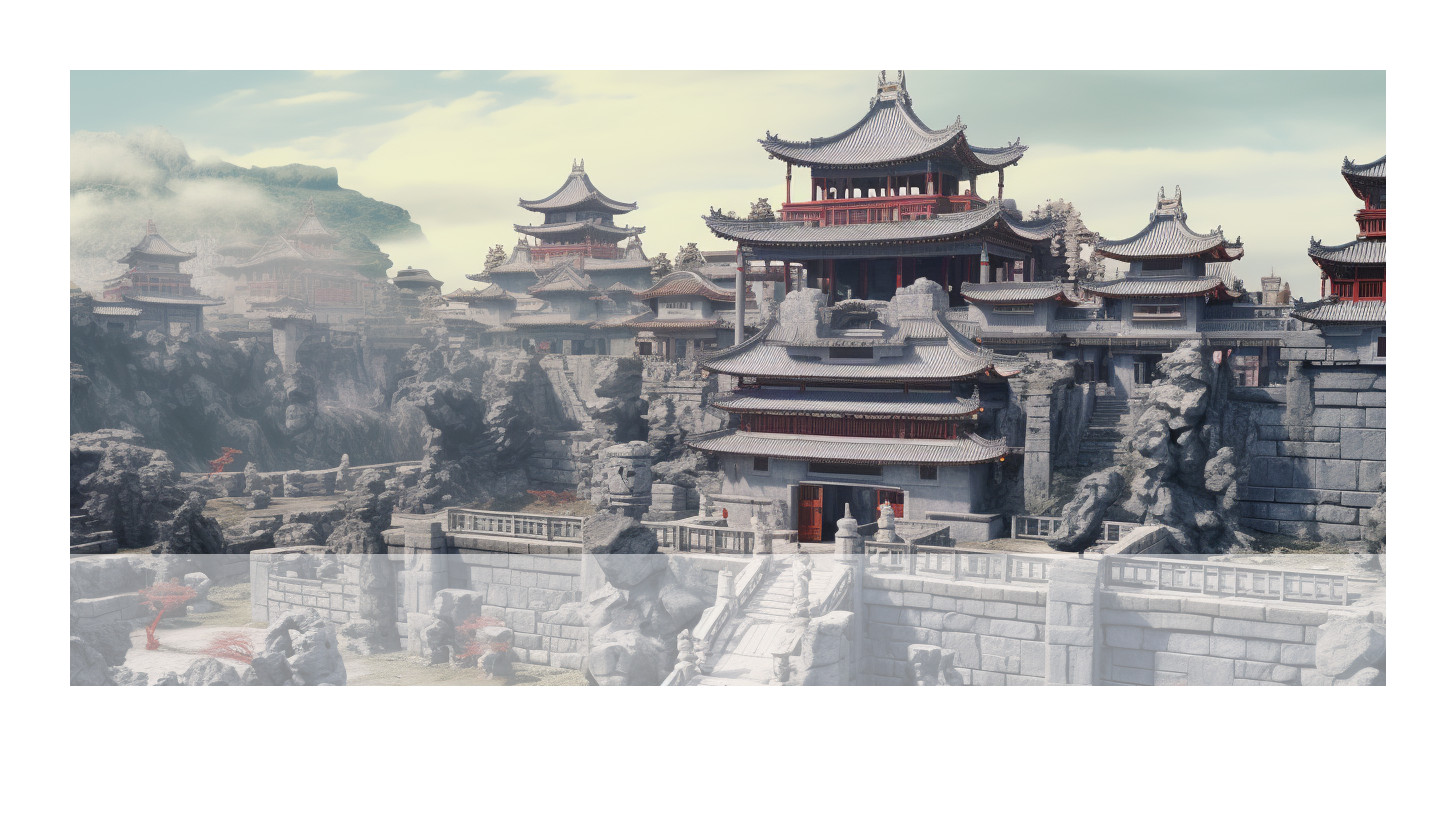
\includegraphics[width=\paperwidth]{./chapters/appendix.jpg}%
    }%
  }
}

%\iniziocapitolo{M}yDevicePolicyManager is a class that wraps DevicePolicyManager and provides a set of methods to manage the device. It is used by the \textit{AdminReceiver} class to perform the operations required by the application.\\

\iniziocapitolo{M}yDevicePolicyManager class is a utility class in the \texttt{com.akhter.siliconlauncher13.tools} package that provides methods and functionalities related to device policy management. It is used to control various device management features on an Android device.

\subsection{Constructor}

\textbf{Constructor:} \texttt{MyDevicePolicyManager(Context context, ComponentActivity activity)}

The constructor for this class takes two parameters: a \texttt{Context} object and a \texttt{ComponentActivity} object. These objects are used to initialize the device policy manager and other components necessary for device management.

\subsection{Methods}

\begin{itemize}
  \item \textbf{addPackageToLockTask(String packageName)}: Adds a specified package to the LockTask mode, allowing it to run exclusively on the device.

  \item \textbf{removePackageFromLockTask(String packageName)}: Removes a specified package from the LockTask mode, allowing it to run like a regular app.

  \item \textbf{startKiosk()}: Initiates the Kiosk mode, which restricts the device to a single app. It also displays a debug toast message.

  \item \textbf{stopKiosk()}: Exits the Kiosk mode and displays a debug toast message.

  \item \textbf{disallowUsbFileTransfer()}: Disallows USB file transfer and mounting of physical media.

  \item \textbf{allowUsbFileTransfer()}: Allows USB file transfer and mounting of physical media.

  \item \textbf{setTethering(boolean allow)}: Allows or disallows tethering based on the specified boolean value.

  \item \textbf{allowScreenCapture()}: Allows screen capture if the app is a device owner.

  \item \textbf{disallowScreenCapture()}: Disallows screen capture if the app is a device owner.

  \item \textbf{setApplicationHidden(String packageName, boolean hidden)}: Sets the hidden state of a specified application.

  \item \textbf{isDeviceOwnerApp()}: Checks if the current app is the device owner.
\end{itemize}

\subsection{Attributes}

\begin{itemize}
  \item \textbf{devicePolicyManager}: An instance of the Android \texttt{DevicePolicyManager} used for device management tasks.

  \item \textbf{adminComponent}\footnote{\label{adminComponentLine}line n. \ref{line:adminComponent}, Listing n. \ref{lst:mydevicepolicymanager}}:  An instance of \texttt{ComponentName} representing the admin receiver component.

  \item \textbf{allowedPackages}: A \texttt{HashSet} containing package names that are allowed to run in LockTask mode.
  \item \textbf{packagesToBeAlwaysEnabled}: In Listing n. \ref{lst:mydevicepolicymanager}, at line n. \ref{line:packagesToBeAlwaysEnabled}, we define an immutable list called `packagesToBeAlwaysEnabled`. This list contains package names that should not be disabled, as doing so could render the system unbootable. When these packages are disabled through the graphical interface by the admin\footnote{\label{administrator}The person with the USB Stick}, they are only prevented from accessing LockTask mode, but they can still run during the TouchPanel boot process. This is a stability measure designed to prevent the admin from completely disabling essential system apps, which could result in an inability to boot the device. If an unprivileged user attempts to launch one of these packages, it will trigger a 'LockTask violation attempt.'
\end{itemize}

\subsection{Constants}

\begin{itemize}
  \item \textbf{TAG}: A constant string representing the tag used for logging purposes.
\end{itemize}

\clearpage

\lstinputlisting[language=Kotlin,linewidth=1\linewidth,caption={MyDevicePolicyManager.kt}, label=lst:mydevicepolicymanager, escapechar=\%]{/home/daniele/akhter/Touchscreen-Lockdown/app/SiliconLauncher13/app/src/main/java/com/akhter/siliconlauncher13/tools/MyDevicePolicyManager.kt}